
\chapter{Problem Statement}
\label{chap:problem_statement}

From the discussion in chapter \ref{chap:problem_statement} it follows that the use of CAN as signalling protocol for  performing OBD-II operations, thereby inheriting all of CAN's security related shortcomings, attributes to a system that is inherently insecure. This chapter serves as a description of the security related problems that arise from the OBD-II specification, as well as providing a series of examples illustrating these problems.

\section{Current State}
\label{sec:current_state}

Figure \ref{fig:topography} shows the typical topography of the OBD-II system. The user interacts with the intra vehicle network via the OBD-II interface using some computerised device (see section \ref{subsec:obd:pid}). The central gateway receives and interprets all messages issued by this device, before forwarding them to the appropriate sub-networks. Optionally, upon reception by the intended ECU, a response could be issued and forwarded back to the user. All of this happens concurrently with the normal operation of the intra vehicle network, i.e. messages are exchanged by ECU's over the entire intra vehicle network to guarantee the optimal operation of the vehicle. The problem of this system is the indiscriminate nature at which the gateway forwards the messages it receives from the OBD-II interface. It does not discern between a normal message and a potentially harmful one. This results in an interface that is rendered wide open to any message that the gateway understands. While in theory, it was designed solely for diagnostic and maintenance purposes. This discrepancy between the intention of the OBD-II design and the wide open nature of it's implementation is apparent. As a result of this, the OBD-II interface can be used to mount a series of attacks. To get a sense of the scope, difficulty and impact of these attacks, a couple of real examples are discussed next.

\begin{figure}[h]
	\label{fig:topography}
	\centering
	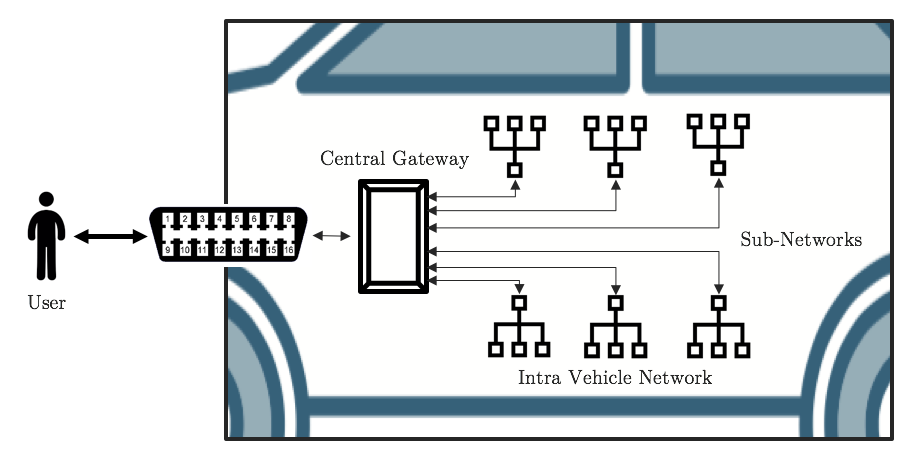
\includegraphics[width=\textwidth]{obd_topography.png}
	\caption{OBD-II System Topography}
\end{figure}

\subsection{Example attacks}
\label{subsec:example_attacks}
The exploits that are presented here were performed by Charlie Miller and Chris Valasek, in an effort to raise awareness about the issue, as well as allowing car manufacturers to build safer cars in the future. They accomplished this by not only finding and exploiting various vulnerabilities in extant vehicles, but also sharing any software that made these exploits possible. An example of this is EcomCat, which is software written to aid in the reading and writing of data to the CAN bus through one or more Ecom cables \cite{MillerC}. The Ecom cable is then used to connect a laptop to the OBD-II DLC, allowing the researchers to use their EcomCat software to inject their own CAN messages onto the internal bus. Although seemingly straightforward there are many potential problems in attempting to make the vehicle perform actions by injecting packets on the CAN bus. First, not everything can be controlled via the CAN bus (e.g. cruise control). Second, if a specific type of CAN packet is found to be a request (An ECU asking for another ECU to perform an action) replaying a fake copy does not guarantee that the message is accepted. This is because the original message is still sent, possibly confusing the ECU with conflicting information. Third, It is also possible that fake messages are ignored because of built-in security features inside the ECU. Despite these difficulties, these researchers did manage to mount a series of interesting exploits, two of which are presented here.

\subsubsection{Speedometer} 
\label{subsec:speedometer}

In this example ,performed on a 2010 Toyota Prius, the researchers managed to identify the messages that are sent to the speedometer to display the current velocity of the vehicle. Replaying this message with custom data fields allowed them to display any arbitrary speed on the speedometer display.

\subsubsection{Denial of Service} 
\label{subsec:denial_of_service}

Here the researches cleverly take advantage of how the CAN protocol works. Remember from \ref{sec:can} that CAN uses priority scheduling over the ID's of the messages that are sent on the bus. This means that spamming a high priority message would prevent all other messages from being transmitted. This vulnerability is exploited here by flooding the bus with CAN messages with an ID of 0. This flooding of the CAN bus halts the engine from being turned on, as well as putting the system in an all out state of disarray.

\subsubsection{Diagnostic session} 
\label{subsec:diagnostic_session}

The aforementioned examples used injection of messages that are normally sent from ECU to ECU, thereby erroneously invoking certain actions. Another approach is to trick the vehicle network into starting a diagnostic session. These are used in normal circumstances by a technician at a garage. It allows them to test the function of an ECU without having to take the vehicle on the road, as well as recalibrating them. Starting a diagnostic session does require circumventing an authentication procedure (see \ref{sec:obd_access_control}) but this proved rather easy (they did this by reverse engineering an official authentication device and extracting the keys). Once a diagnostic session was established it opened up a wide array of possible attacks: Killing the engine, disabling the brakes, honking the horn, unlocking/locking doors, and even reprogramming of certain ECU's (see \cite{MillerC} for a detailed description of the attacks).

\subsection{Impact}
\label{subsec:impact}

It is clear that the level of control that is obtainable via the OBD-II port is worrying. Especially if we consider that there exist OBD-II devices with Bluetooth or Wifi capabilities, allowing attacks to be mounted from a distance (imagine a DoS attack being mounted while driving a car at high speed). It is these scenarios that elevate the concern from mere vehicular integrity, to concern over the physical safety of the driver and his/her passengers. Sure it could be stated that this danger originates from a malicious agent gaining illegal access to the vehicle, rather than the security of the internal vehicle system. But this assertion would gloss over the fact that the OBD-II interface was designed to be used only by repairman, testers, policemen, etc. Therefore it is only logical that this privileged use is enforced by the system, rather than being merely implied.

\section{Attacker model} 
\label{sec:attacker_model}
Here, an attempt is made to define the types of attackers that this paper aims to defend against. a similar classification as \cite{Maxim} and \cite{Petit} is followed:

\begin{itemize}
	\item \textbf{Insider or outsider:} The insider is considered an interactive member of the network, meaning he/she can communicate with other members freely. The outsider however is limited in the diversity of attacks he/she can mount.
	
	Classification: \textbf{outsider}, since the attacker is not part of the CAN bus. It is worth noting however that when the attacker uses the OBD port to mount an attack, he/she can communicate with the other nodes on the bus. This however is treated by this paper as part of a successful attack, not as an a priori capability of the attacker.
	
	\item \textbf{Malicious or rational:}  A malicious attacker exploits the system for reasons other than personal gain, making them more unpredictable since their motives and resources can vary. A rational attacker however is motivated solely by personal profit, be it money or fame, making them more predictable.
	
	Classification: \textbf{both}, since an attacker using the OBD port as attack vector could be both malicious (e.g. Endangering the life of a rival) and rational (e.g. lowering the internal odometer value before selling the vehicle).
	
	\item \textbf{Active or passive:} An active attacker is able to generate and transmit messages, whereas a passive attacker is constrained to eavesdropping.
	
	Classification: \textbf{active}, since we know the attacker can have access to tools (e.g. PassThru) that grant him/her active capabilities.
	
	\item \textbf{Local or extended:} This criterion is based on the scope of the attacker. A local attacker has only limited attack vectors, whereas an extended attacker has access to lots.
	
	Classification: \textbf{local}, since a comprehensive analysis of multiple attack vectors, although touched upon in section \ref{sec:other_attack_vectors}, is considered out of scope for this paper (c.f. \cite{Pike15}\cite{Kleberger15}\cite{Russel17}\cite{MillerA}\cite{Petit}\cite{Kosher}\cite{Kosher2}\cite{Bayer15}).
\end{itemize}

